\chapter{Resultate und Testen} \label{chap:resultate}

\section{Testen} \label{sec:testen}

Die Webseite lässt sich testen in einer lokalen Entwicklungsumgebung oder auf
der öffentlichen Seite. Getestet wurden die Funktionen manuell von Hand oder
durch automatisierte Tests.

Grundsätzlich funktionieren alle Funktionen. Schlussendlich gibt es nur ein
Problem: Es kommt vor, dass der Webscraper Edge-Cases antrifft. Das kann
passieren, wenn die offizielle Mensa Webseite die Informationen auf ihrer
Webseite kurzfristig ändern. Es wurde versucht diese Edge-Cases möglichst alle
abzufangen, allerdings kann es immer noch sein, dass es manchmal zu Fehlern
kommt. Diese Fehler müssten dann von einem Admin auf der Admin-Seite behoben
werden.

\section{Resultate} \label{sec:resultate}

Als Resultat dieser Arbeit ist eine voll funktionsfähige Webseite entstanden.
Die Webseite erfüllt alle nötigen Anforderungen (siehe
\ref{sec:problemdefinition}). Die Webseite ist auch öffentlich zugänglich
(siehe \ref{spez:Deployment}) und kann unter
\url{http://mensarating.herokuapp.com/} aufgerufen werden. Es lässt sich also
sagen, dass die Webseite komplett einsatzbereit ist und Nutzer von der NKSA sie
beginnen können zu benutzen.

\subsection{Resultate der Grundanforderungen}
 
\newpage

\subsubsection*{Anzeige der Menus}

\begin{figure}[ht]
    \centering
    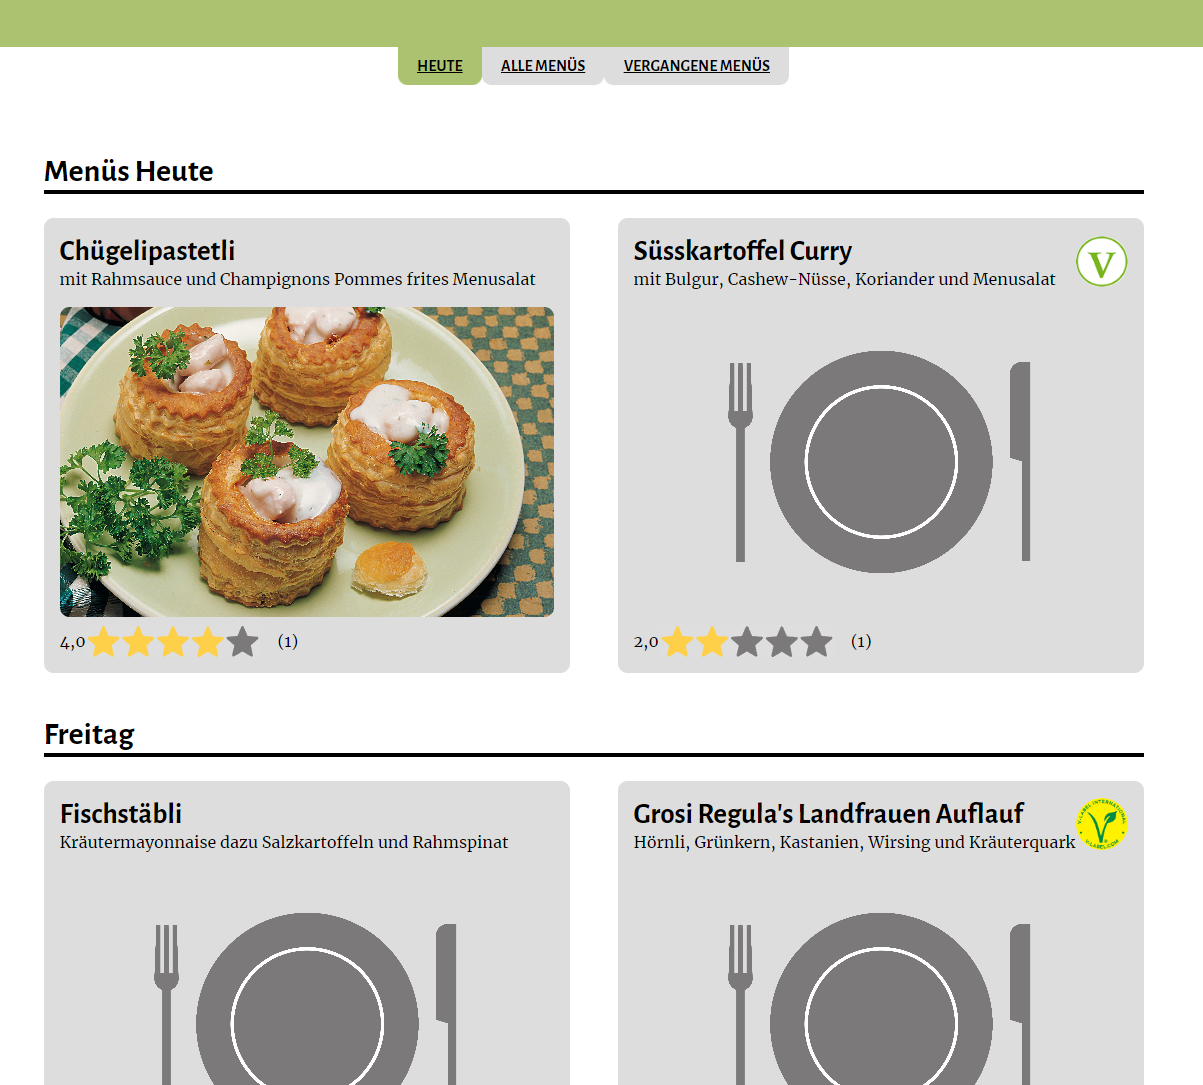
\includegraphics[width=0.8\textwidth]{images/Resultate_Menu.png}
    \caption{Screenshot: Anzeige Menus auf Startseite}
    \label{fig:r-menuindex}
\end{figure}

Auf der Startseite der Webseite (siehe \ref{fig:r-menuindex}) werden die beiden Menus des Tages, die von der
offiziellen Mensa Webseite gescraped wurden, angezeigt. Es wird die
Beschreibung, ein Label (Vegan/Vegetarisch), das durchschnittliche Rating und
das Bild mit den meisten Likes angezeigt. Als Zusatz sind die zukünftigen Menus
ebenfalls angezeigt

\begin{figure}[htp]
    \begin{subfigure}[b]{0.5\textwidth}
        \centering
        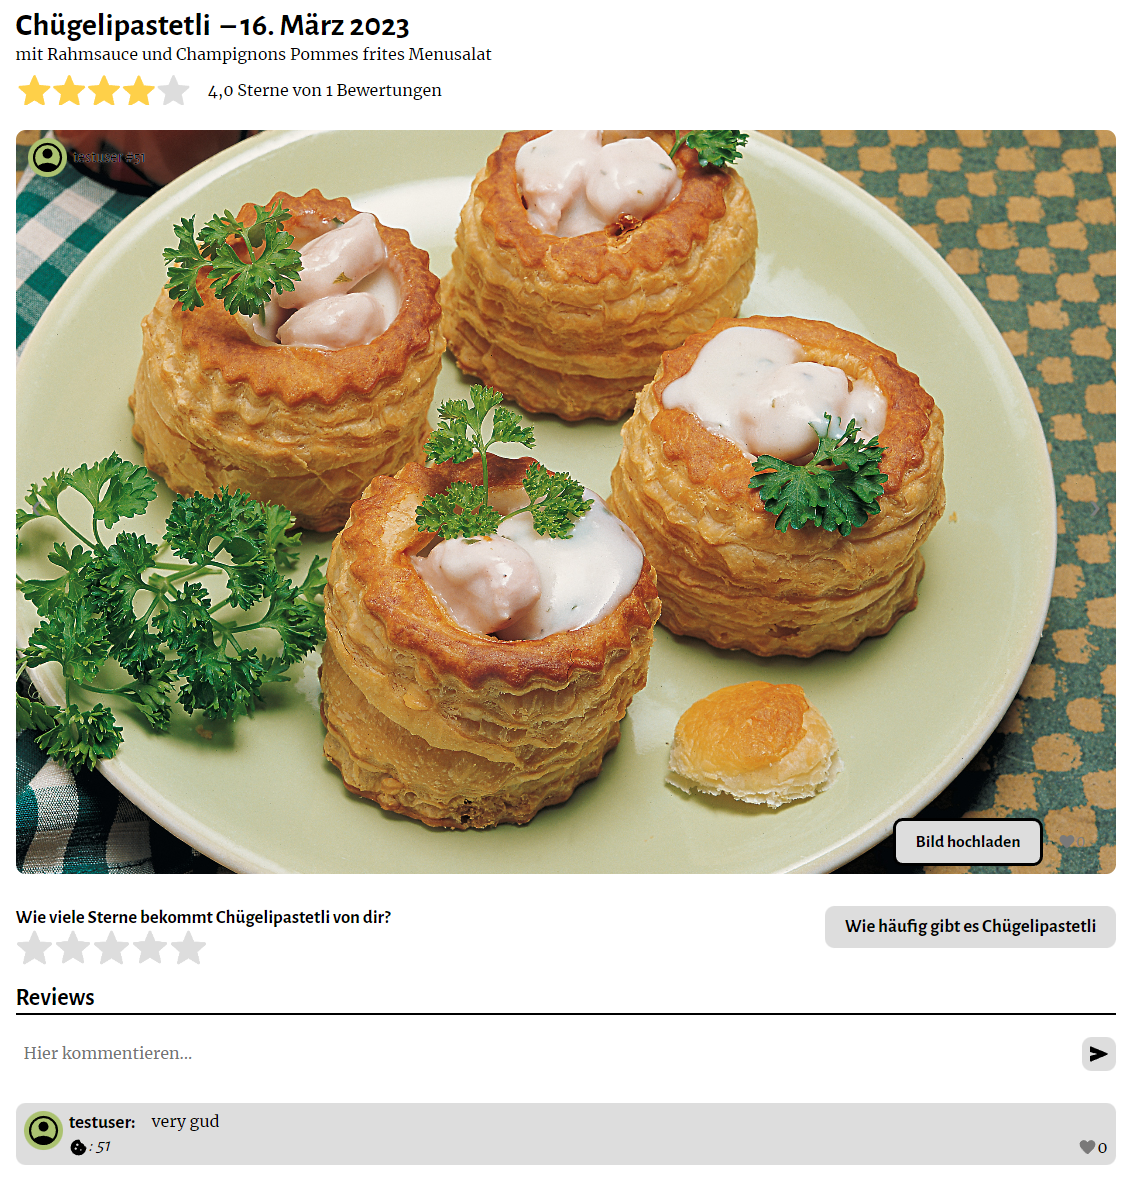
\includegraphics[width=0.7\textwidth]{images/Res_Menu.png}
        \caption{Screenshot: Menu Web Page}
        \label{fig:r-menu}
    \end{subfigure}
    \begin{subfigure}[b]{0.5\textwidth}
        \centering
        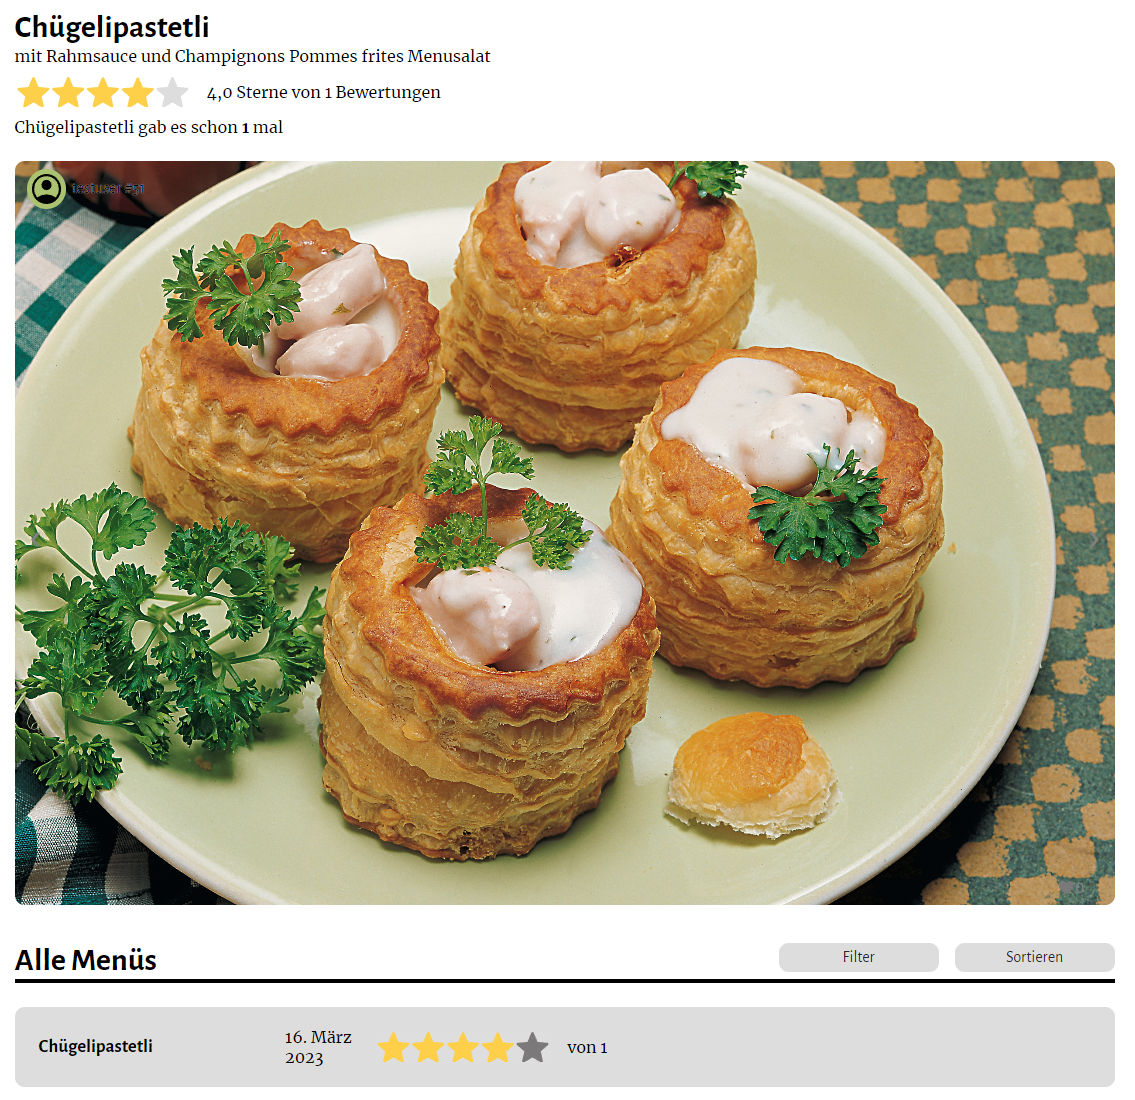
\includegraphics[width=0.7\textwidth]{images/Res_Menutype.png}
        \caption{Screenshot: Menutype Web Page}
        \label{fig:r-menutype}
    \end{subfigure}
    \hfill
\end{figure}

Zusätzlich gibt es eine Menu Page (siehe \ref{fig:r-menu}) und eine MenuType
Page (siehe \ref{fig:r-menutype}), wo die Menus genauer angezeigt werden  


\subsubsection*{Bilder Gallerie}

\begin{figure}[htp]
    \begin{subfigure}[b]{0.5\textwidth}
        \centering
        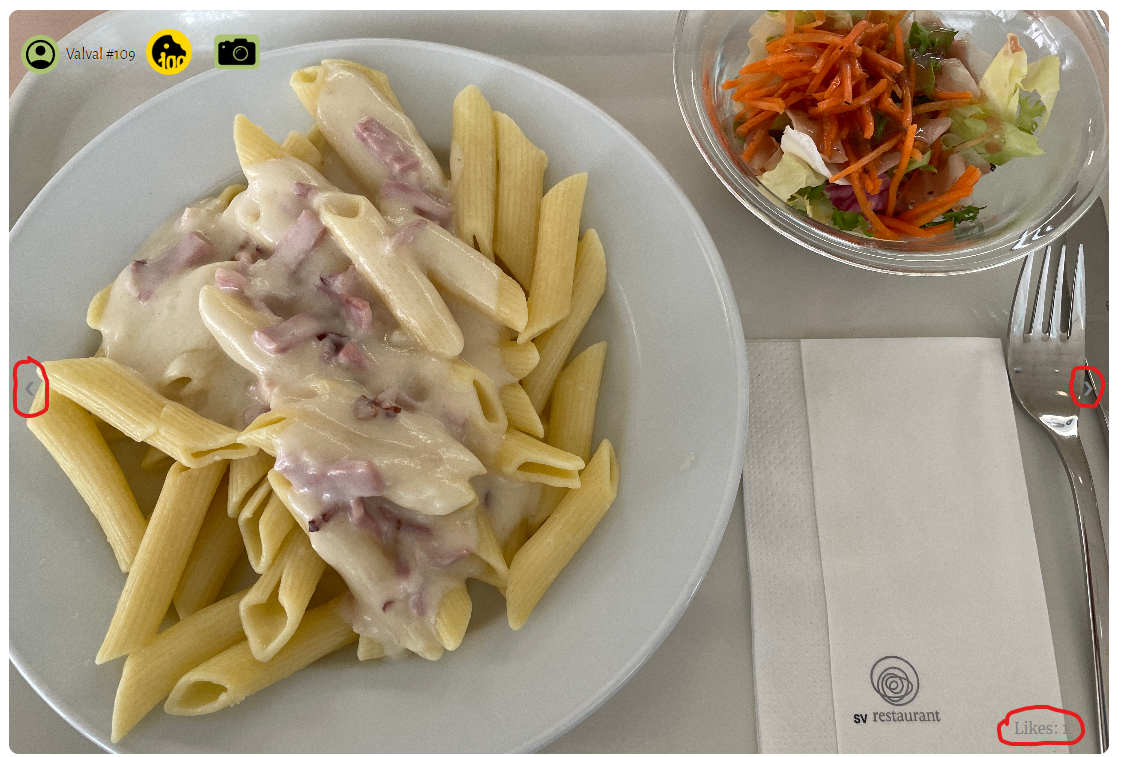
\includegraphics[width=0.7\textwidth]{images/Resultate_Bildergallerie.png}
        \caption{Screenshot: Bildergallerie}
        \label{fig:r-bildergallerie}
    \end{subfigure}
    \begin{subfigure}[b]{0.5\textwidth}
        \centering
        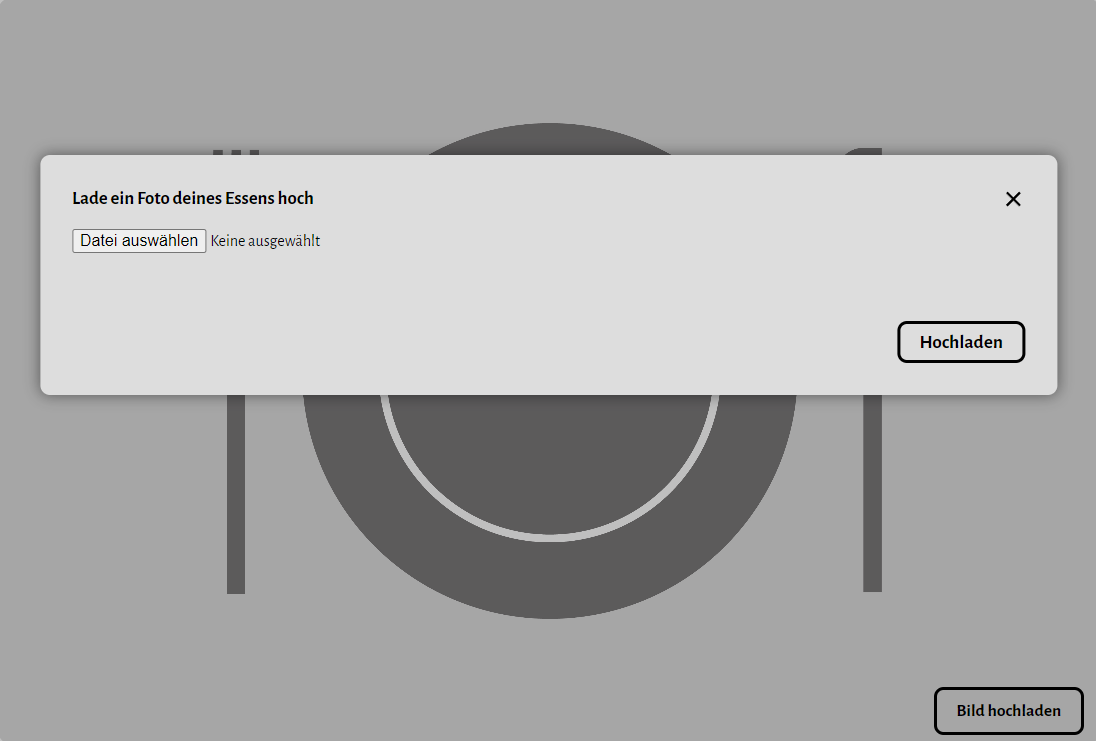
\includegraphics[width=0.7\textwidth]{images/Resultat_Bildergallerie_upload.png}
        \caption{Screenshot: Bilder Upload}
        \label{fig:r-bildpopup}
    \end{subfigure}
    \hfill
\end{figure}

Bei der Bildergallerie (siehe \ref{fig:r-bildergallerie}) können User Bilder
hochladen. Man kann durch Pfeil-Buttons die hochgeladenen Bilder durchschauen.
Für ein Bild ist der User angezeigt, der es hochgeladen hat, und die Anzahl
likes. Der Upload findet über einen Upload Button statt, der ein Pop-Up öffnet
(siehe \ref{fig:r-bildpopup})


\subsubsection*{Reviews}

\begin{figure}[ht]
    \centering
    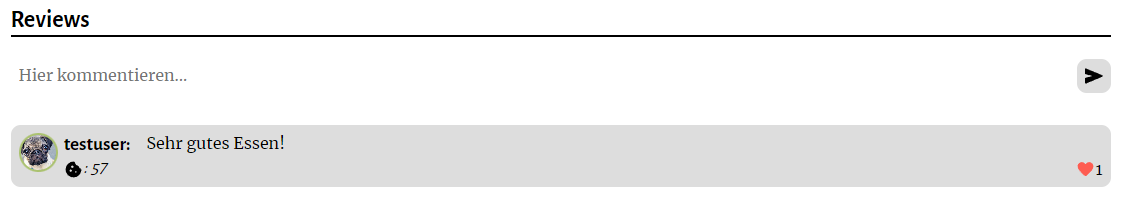
\includegraphics[width=0.8\textwidth]{images/Resultat_Review.png}
    \caption{Screenshot: Veröffentlichung und Anzeige von Reviews}
    \label{fig:r-review}
\end{figure}

Am Tag, an dem es ein Menu gibt, kann diesem Menu ein Review (siehe \ref{fig:r-review}) gegeben werden. Die
Reviews sind in einer Liste angeordet und bei jedem Review ist der User
angegeben, zusammen mit seinen Achievements und Karma Punkten. Reviews können
geliked werden (Beachte das Herz).


\subsubsection*{Rating}
\subsubsection*{Filtern/Sortieren}
\subsubsection*{Design}

\subsection{Resultate der Erweiterungskriterien}

\subsubsection*{Account System}
\subsubsection*{Mobile Responsiveness}
\subsubsection*{Punktesystem (Karma)}
\subsubsection*{Likes}
\subsubsection*{Achievement System}
\subsubsection*{Deployment}







